%-----------------------------------------------------------------------------
%
%               Template for sigplanconf LaTeX Class
%
% Name:         sigplanconf-template.tex
%
% Purpose:      A template for sigplanconf.cls, which is a LaTeX 2e class
%               file for SIGPLAN conference proceedings.
%
% Guide:        Refer to "Author's Guide to the ACM SIGPLAN Class,"
%               sigplanconf-guide.pdf
%
% Author:       Paul C. Anagnostopoulos
%               Windfall Software
%               978 371-2316
%               paul@windfall.com
%
% Created:      15 February 2005
%
%-----------------------------------------------------------------------------


\documentclass[preprint]{sigplanconf}

% The following \documentclass options may be useful:

% preprint      Remove this option only once the paper is in final form.
% 10pt          To set in 10-point type instead of 9-point.
% 11pt          To set in 11-point type instead of 9-point.
% authoryear    To obtain author/year citation style instead of numeric.

\usepackage{amsmath}
\usepackage{listings,xspace}
\usepackage{amsthm}
\usepackage{mdframed}
\usepackage{xcolor}
\usepackage{fontspec}
\usepackage{graphicx}
\usepackage{setspace}
% \usepackage{booktabs}
\usepackage{wasysym}
\usepackage{amsthm}
\usepackage{url}

\usepackage{caption}
\usepackage{subcaption}

\usepackage{csquotes}
\usepackage{enumitem}
\usepackage{todonotes}

% \usepackage{bcprules}
% \usepackage{prooftree}
\usepackage{multicol}

\lstdefinelanguage{Scala}%
{morekeywords={abstract,case,catch,char,class,%
    def,else,extends,final,%
    if,import,%
    match,module,new,null,object,override,package,private,protected,%
    public,return,super,this,throw,trait,try,type,val,var,with,implicit,%
    macro,sealed,%
  },%
  sensitive,%
  morecomment=[l]//,%
  morecomment=[s]{/*}{*/},%
  morestring=[b]",%
  morestring=[b]',%
  showstringspaces=false%
}[keywords,comments,strings]%

\lstset{language=Scala,%
  mathescape=true,%
  columns=[c]fixed,%
  basewidth={0.5em, 0.40em},%
  basicstyle=\tt,%
  commentstyle=\color{gray}\itshape\ttfamily,
  xleftmargin=0.0cm
}

% \lstset{tabsize=2,
% basicstyle=\ttfamily\fontsize{9pt}{1em}\selectfont,
% commentstyle=\color{gray}\itshape\ttfamily,
% numbers=left, numberstyle=\scriptsize\color{gray}\ttfamily, language=scala,moredelim=[il][\sffamily]{?},mathescape=false,showspaces=false,showstringspaces=false,xleftmargin=15pt,escapechar=@, morekeywords=[1]{let,fn,val},deletekeywords={for},classoffset=0,belowskip=\smallskipamount
% }

\theoremstyle{definition}
\newmdtheoremenv[hidealllines=true,topline=true,bottomline=true,skipabove=\baselineskip,skipbelow=\baselineskip]{defn}{Definition}[section]

\theoremstyle{definition}
\newmdtheoremenv[hidealllines=true,topline=true,bottomline=true,skipabove=\baselineskip,skipbelow=\baselineskip]{prop}{Property}[section]

% \theoremstyle{nonumberplain}
% \theoremstyle{definition}
% \newmdtheoremenv*[hidealllines=true,topline=true,bottomline=true,skipabove=\baselineskip,skipbelow=\baselineskip]{defnn}{Definition}[section]
\newtheorem*{defn*}{Definition}

% \newtheorem{defn}{Definition}[section]
% \newenvironment{defn}
  % {\begin{mdframed}[style=warning]\begin{mdef}}
  % {\end{mdef}\end{mdframed}}

% comments and notes
\newcommand{\comment}[1]{}
\newcommand{\note}[1]{{\bf $\clubsuit$ #1 $\spadesuit$}}
\newcommand{\ifreport}[1]{#1}
%\newcommand{\ifreport}[1]{}

\newcommand{\ie}{{\em i.e.,~}}
\newcommand{\eg}{{\em e.g.,~}}
\newcommand{\term}[1]{\mbox{\texttt{#1}}}
\newcommand{\itl}[1]{\mbox{\textit{#1}}}

% commas and semicolons
\newcommand{\comma}{,\,}
\newcommand{\commadots}{\comma \ldots \comma}
\newcommand{\semi}{;\mbox{;};}
\newcommand{\semidots}{\semi \ldots \semi}

% spacing
\newcommand{\gap}{\quad\quad}
\newcommand{\biggap}{\quad\quad\quad}
\newcommand{\nextline}{\\ \\}
\newcommand{\htabwidth}{0.5cm}
\newcommand{\tabwidth}{1cm}
\newcommand{\htab}{\hspace{\htabwidth}}
\newcommand{\tab}{\hspace{\tabwidth}}
\newcommand{\linesep}{\ \hrulefill \ \smallskip}

\newcommand{\sectionline}{%
  \nointerlineskip \vspace{\baselineskip}%
  \hspace{\fill}\rule{0.5\linewidth}{.7pt}\hspace{\fill}%
  \par\nointerlineskip \vspace{\baselineskip}
}

% figures
\newcommand{\figurebox}[1]
        {\fbox{\begin{minipage}{\textwidth} #1 \medskip\end{minipage}}}
\newcommand{\twofig}[3]
        {\begin{figure*}[t]#3\ \hrulefill\
        \caption{\label{#1}#2}\end{figure*}}
\newcommand{\boxfig}[3]
        {\begin{figure*}\figurebox{#3\caption{\label{#1}#2}}\end{figure*}}
\newcommand{\figref}[1]
        {Figure~\ref{#1}}

% arrays
\newcommand{\ba}{\begin{array}}
\newcommand{\ea}{\end{array}}
\newcommand{\bda}{\[\ba}
\newcommand{\eda}{\ea\]}
\newcommand{\ei}{\end{array}}
\newcommand{\bcases}{\left\{\begin{array}{ll}}
\newcommand{\ecases}{\end{array}\right.}

%%%%%%%%%%%%%%%%%%%%%%%%%%%%%%%%%%%%%%%
%   Language abstraction commands     %
%%%%%%%%%%%%%%%%%%%%%%%%%%%%%%%%%%%%%%%

%% Relations
% Subtype
\newcommand{\sub}{<:}
% Type assignment
\newcommand{\typ}{:}
% reduction
\newcommand{\reduces}{\;\rightarrow\;}
% well-formedness
\newcommand{\wf}{\;\mbox{\textbf{wf}}}

%% Operators
% Type selection
\newcommand{\tsel}{\#}
% Function type
\newcommand{\tfun}{\rightarrow}
\newcommand{\dfun}[3]{(#1\!:\!#2) \Rightarrow #3}
% Conjunction
\newcommand{\tand}{\wedge}
% Disjunction
\newcommand{\tor}{\vee}
% Singleton type suffix
\newcommand{\sing}{.\textbf{type}}

%% Syntax
% Header for typing rules
\newcommand{\judgement}[2]{{\bf #1} \hfill \fbox{#2}}
% Refinement
\newcommand{\refine}[2]{\left\{#1 \Rightarrow #2 \right\}}
% Field definitions
\newcommand{\ldefs}[1]{\left\{#1\right\}}
% Member sequences
\newcommand{\seq}[1]{\overline{#1}}
% Lambda
\newcommand{\dabs}[3]{(#1\!:\!#2)\Rightarrow #3}
\newcommand{\abs}[3]{\lambda #1\!:\!#2.#3}
% Application
\newcommand{\app}[2]{#1\;#2}
% Substitution
\newcommand{\subst}[3]{[#1/#2]#3}
% Object creation
\newcommand{\new}[3]{\textbf{val }#1 = \textbf{new }#2 ;\; #3}
%\renewcommand{\new}[3]{#1 \leftarrow #2 \,\textbf{in}\, #3}
% Field declaration
\newcommand{\Ldecl}[3]{#1 \typ #2..#3}%{#1 \operatorname{>:} #2 \operatorname{<:} #3}
\newcommand{\ldecl}[2]{#1 \typ #2}
% Top and Bottom
\newcommand{\Top}{\top}%{\textbf{Top}}
\newcommand{\Bot}{\bot}%\textbf{Bot}}
% Environment extension
\newcommand{\envplus}[1]{\uplus \{ #1 \}}

\newcommand{\reduction}[4]{#1, #2 \reduces #3, #4}
\newcommand{\reducebig}[6]{#1, #2, #3 \;\Downarrow\; #4, #5, #6}
\newcommand{\evaluate}[5]{#1, #2, #3 \;\Downarrow\; #4, #5}
\newcommand{\evalcap}[8]{#1, #2, #3, #4 \;\Downarrow\; #5, #6, #7, #8}
\newcommand{\evalcapbreak}[8]{#1, #2, #3, #4 \;\Downarrow\; \\ #5, #6, #7, #8}
\newcommand{\evalcapfin}[9]{#2, #3, #4, #5 \;\Downarrow_{#1}\; #6, #7, #8, #9}

\newcommand{\sframe}[3]{\langle #1, #2, #3 \rangle}
\newcommand{\stack}[4]{#1 \sframe {#2} {#3} {#4}}
\newcommand{\reduce}[4]{#1, #2 \;\longrightarrow\; #3, #4}
\newcommand{\reducebreak}[4]{#1, #2 \\ \;\longrightarrow\; #3, #4}

\newcommand{\sreduce}[6]{#1, #2, #3 \;\longrightarrow\; #4, #5, #6}
\newcommand{\sreducebreak}[6]{#1, #2, #3 \\ \;\longrightarrow\; #4, #5, #6}
\newcommand{\sreducestar}[6]{#1, #2, #3 \;\longrightarrow^{\ast}\; #4, #5, #6}
\newcommand{\sreducestarbreak}[6]{#1, #2, #3 \\ \;\longrightarrow^{\ast}\; #4, #5, #6}

% misc identifiers
\newcommand{\dom}{\mbox{\sl dom}}
\newcommand{\fn}{\mbox{\sl fn}}
\newcommand{\bn}{\mbox{\sl bn}}
\newcommand{\sig}{\mbox{\sl sig}}
\newcommand{\IF}{\mbox{\mathem if}}
\newcommand{\OTHERWISE}{\mbox{\mathem otherwise}}
\newcommand{\strongexpand}{\prec\!\!\prec}
\newcommand{\weakexpand}{\prec}
\newcommand{\spcomma}{~,~}

% hide the copyright box
% \makeatletter
% \def\@copyrightspace{\relax}
% \makeatother


\begin{document}

\special{papersize=8.5in,11in}
\setlength{\pdfpageheight}{\paperheight}
\setlength{\pdfpagewidth}{\paperwidth}

\setmainfont[Mapping=tex-text]{Times New Roman}
\setmonofont[Scale=0.8,BoldFont={Consolas Bold}]{Consolas}

\conferenceinfo{CONF 'yy}{Month d--d, 20yy, City, ST, Country}
\copyrightyear{20yy}
\copyrightdata{978-1-nnnn-nnnn-n/yy/mm}
\doi{nnnnnnn.nnnnnnn}

% Uncomment one of the following two, if you are not going for the
% traditional copyright transfer agreement.

%\exclusivelicense                % ACM gets exclusive license to publish,
                                  % you retain copyright

%\permissiontopublish             % ACM gets nonexclusive license to publish
                                  % (paid open-access papers,
                                  % short abstracts)

% \titlebanner{banner above paper title}        % These are ignored unless
% \preprintfooter{short description of paper}   % 'preprint' option specified.

% \title{Function-Passing Style: A Functional Model of Concurrent Computation for Distributed Systems}
\title{Function-Passing Style: A Model for Typed, Distributed Functional Programming}
% \title{Function-Passing Style: Typed, Distributed Functional Programming}
% \subtitle{Subtitle Text, if any}

\authorinfo{Heather Miller}
           {EPFL}
           {heather.miller@epfl.ch}
\authorinfo{Philipp Haller}
           {KTH Royal Institute of Technology}
           {phaller@kth.se}

\maketitle

\begin{abstract}
This is the text of the abstract.
\end{abstract}

\category{D.3.3}{Programming Languages}{Language Constructs and Features}

% general terms are not compulsory anymore,
% you may leave them out
\terms
Languages, Design

\keywords
programming languages, functional programming, distributed programming,
functions, closures, serialization, concurrency, types, Scala

\section{Introduction}


Functional programming concepts are making inroads in hot up-and-coming
frameworks for distributed computing and, dare we say it, ``big data.''
Arguably, MapReduce was one of the first systems to pick up FP concepts,
albeit outside the context of functional languages. More recent frameworks are
now also leveraging classical functional language features, such as higher-
order functions (e.g., Spark). This is a boon for mathematically-oriented data
analytics and higher-order functions provide flexible abstraction mechanisms.

However, to provide fault tolerance in the context of large-scale distributed
computing, such frameworks for distribution are built atop of tall stacks of
code which is typically imperative and untyped, losing most of the benefits
enjoyed by the users of their high-level APIs. [What's more,] the benefits of
FP, abstraction, composition, equational reasoning, are seemingly lost by
engineers building these distributed systems. What makes this problem even
worse is the fact that coordinating between data shards and doing that in a
way that is easy to reason about is the wheel that every data-centric
distributed system keeps reinventing.

Fortunately, FP techniques are not only useful for designing good user-facing
APIs. This paper presents a deep connection between the pillars of FP and one
of the most important challenges of distributed computing: fault tolerance. To
this end we present a new programming model for typed distributed functional
programming. This model aims to:

\begin{itemize}
\item distill existing fault recovery mechanisms based on lineage to their essence.
Importantly, this paper shows that there is a direct correspondence between
the concept of lineage, as it is widely used in distributed systems, and well-known
pillars of FP. Our distributed programming model is a consequent
implementation of this correspondence, and demonstrates it in executable form
in the context of an implementation in and for Scala.

\item improve type-safety at the boundary of serialized and deserialized data.
Importantly, the design and implementation of our programming model shows that
even the layer in a distributed system that processes freshly deserialized
data (typically, this layer sits right on top of the network communication
layer) can not only be written in a strongly-typed way, but it can even
leverage performance improvements due to type-specialized serialization.
\end{itemize}

Our programming model is centered around a new distributed persistent data
structure, the silo. A silo is a typed container for a single (immutable)
value. A silo is ``stationary''; it is never moved away from the host on which
it was created. Computations on silos are expressed using SiloRefs, proxy
objects representing remote silos. The primary means to operate on a silo is
by passing a serializable closure to it using a SiloRef. SiloRefs provide a
standard monadic interface as well as primitives for defining flexible fault
handling strategies.

To ensure safe and efficient distribution of closures, our model leverages
both syntactic and type-based restrictions. For instance, closures sent to
remote silos are required to conform to the restrictions imposed by the so-called
``spore'' abstraction~\cite{Spores}. Among others, the syntax and
static semantics of spores guarantees the absence of runtime serialization
errors due to closure environments that are not serializable.

The specific technical contributions of this paper are:

\begin{itemize}
\item A new programming model for functional processing of distributed data. By
leveraging safe serializable closures, it prevents common usage errors of
other widely-used data analytics stacks.

\item A new model of lineage-based fault recovery based on typed FP. Our approach
extends the capabilities of existing implementations by supporting type-specialized,
statically-generated serializers even in the context of
existentially-quantified types.

\item A complete, distributed implementation of the model in Scala.

\item A validation of spores in the context of distributed programming.

\item Self-describing pickles?

\item An experimental evaluation.
\end{itemize}

Closely related work here.

Structure. Our approach is to describe our model from a high level,
elaborating upon key concepts. While focusing on .. over time. We then proceed
to zoom in and make precise each component of our model in Sections~\ref{}.

\section{Overview of Model}

The best way to quickly visualize the F-P model is to think in terms of a
persistent functional data structure with structural sharing. Then, rather
than containing pure data, imagine instead that the structure represents a
directed acyclic graph (DAG) of transformations on distributed data.

Importantly, since this DAG of computations is a persistent data structure
itself, it is safe to exchange (copies of) subgraphs of a DAG between remote
nodes. This enables a robust and easy-to-reason-about model of fault
tolerance. We call subgraphs of a DAG lineages; lineages enable restoring the
data of failed nodes through re-applying the transformations represented by
their DAG. This sequence of applications must begin with data available from
stable storage.

Central to our model is the careful use of laziness. Computations on
distributed data are typically not executed eagerly; instead, applying a
function to distributed data just creates an immutable lineage. To obtain the
result of a computation, it is necessary to first ``kick off'' computation, or
to force its lineage. Within our programming model, this force
operation\todo{which force operation?} makes network communication (and thus
possibilities for latency) explicit, which is considered to be a strength when
designing distributed systems~\cite{ANoteDistComp}. Deferred evaluation also
enables optimizing distributed computations through operation fusion, which
avoids the creation of unnecessary intermediate data structures--this is
efficient in time as well as space. This kind of optimization is particularly
important and effective in distributed systems~\cite{FlumeJava}.\todo{What
does this have to do with FlumeJava?}

\vspace{-3mm}
\begin{center}\noindent\rule{8cm}{0.4pt}\end{center}
\begin{displayquote}
For these reasons, we believe that laziness should be viewed as an enabler in
the design of distributed systems.
\end{displayquote}
\vspace{-4mm}
\begin{center}\noindent\rule{8cm}{0.4pt}\end{center}
\vspace{1mm}

\noindent The F-P model consists of three main components:
\begin{itemize}[noitemsep]
  \item {\bf Silos:} stationary typed data containers.
  \item {\bf SiloRefs:} references to local or remote Silos.
  \item {\bf Spores:} safe, serializable functions.
\end{itemize}
\vspace{1mm}

\paragraph{Silos}
A silo is a typed data container. It is stationary in the sense that it does
not move between machines -- it remains on the machine where it was created.
Data stored in a silo is typically loaded from stable storage, such as a
distributed file system. A program operating on data stored in a silo can only
do so using a reference to the silo, a \verb|SiloRef|.

\paragraph{SiloRefs}
Similar to a proxy object, a SiloRef represents, and allows interacting with,
both local and remote silos. SiloRefs are immutable, storing identifiers to
locate possibly remote silos. SiloRefs are also typed (\verb|SiloRef[T]|)
corresponding to the type of their silo's data, leading to well-typed network
communication. The SiloRef provides three primitive operations/combinators
(some are lazy, some are not): map, flatMap, and send. map lazily applies a
user-defined function to data pointed to by the SiloRef, creating in a new
silo containing the result of this application. Like map, flatMap lazily
applies a user-defined function to data pointed to by the SiloRef. Unlike map,
the user-defined function passed to flatMap returns a SiloRef whose contents
is transferred to the new silo returned by flatMap. Essentially, flatMap
enables accessing the contents of (local or remote) silos from within remote
computations. We illustrate these primitives in more detail in Section~\ref{sec:primitives}.

\paragraph{Spores}

Spores~\cite{Spores} are safe closures that are guaranteed to be serializable
and thus distributable. They are a closure-like abstraction and type system
which gives authors of distributed frameworks a principled way of controlling
the environment which a closure (provided by client code) can capture. This is
achieved by (a) enforcing a specific syntactic shape which dictates how the
environment of a spore is declared, and (b) providing additional type-checking
to ensure that types being captured have certain properties.

\vspace{3mm}
\noindent A spore consists of two parts:

\begin{itemize}[noitemsep]
\item {\bf the spore header}, composed of a list of value definitions.
\item {\bf the spore body} (sometimes referred to as the “spore closure”), a regular closure.
\end{itemize}

\noindent This shape is illustrated below.

\vspace{-1mm}
\begin{figure}[h!]
\centering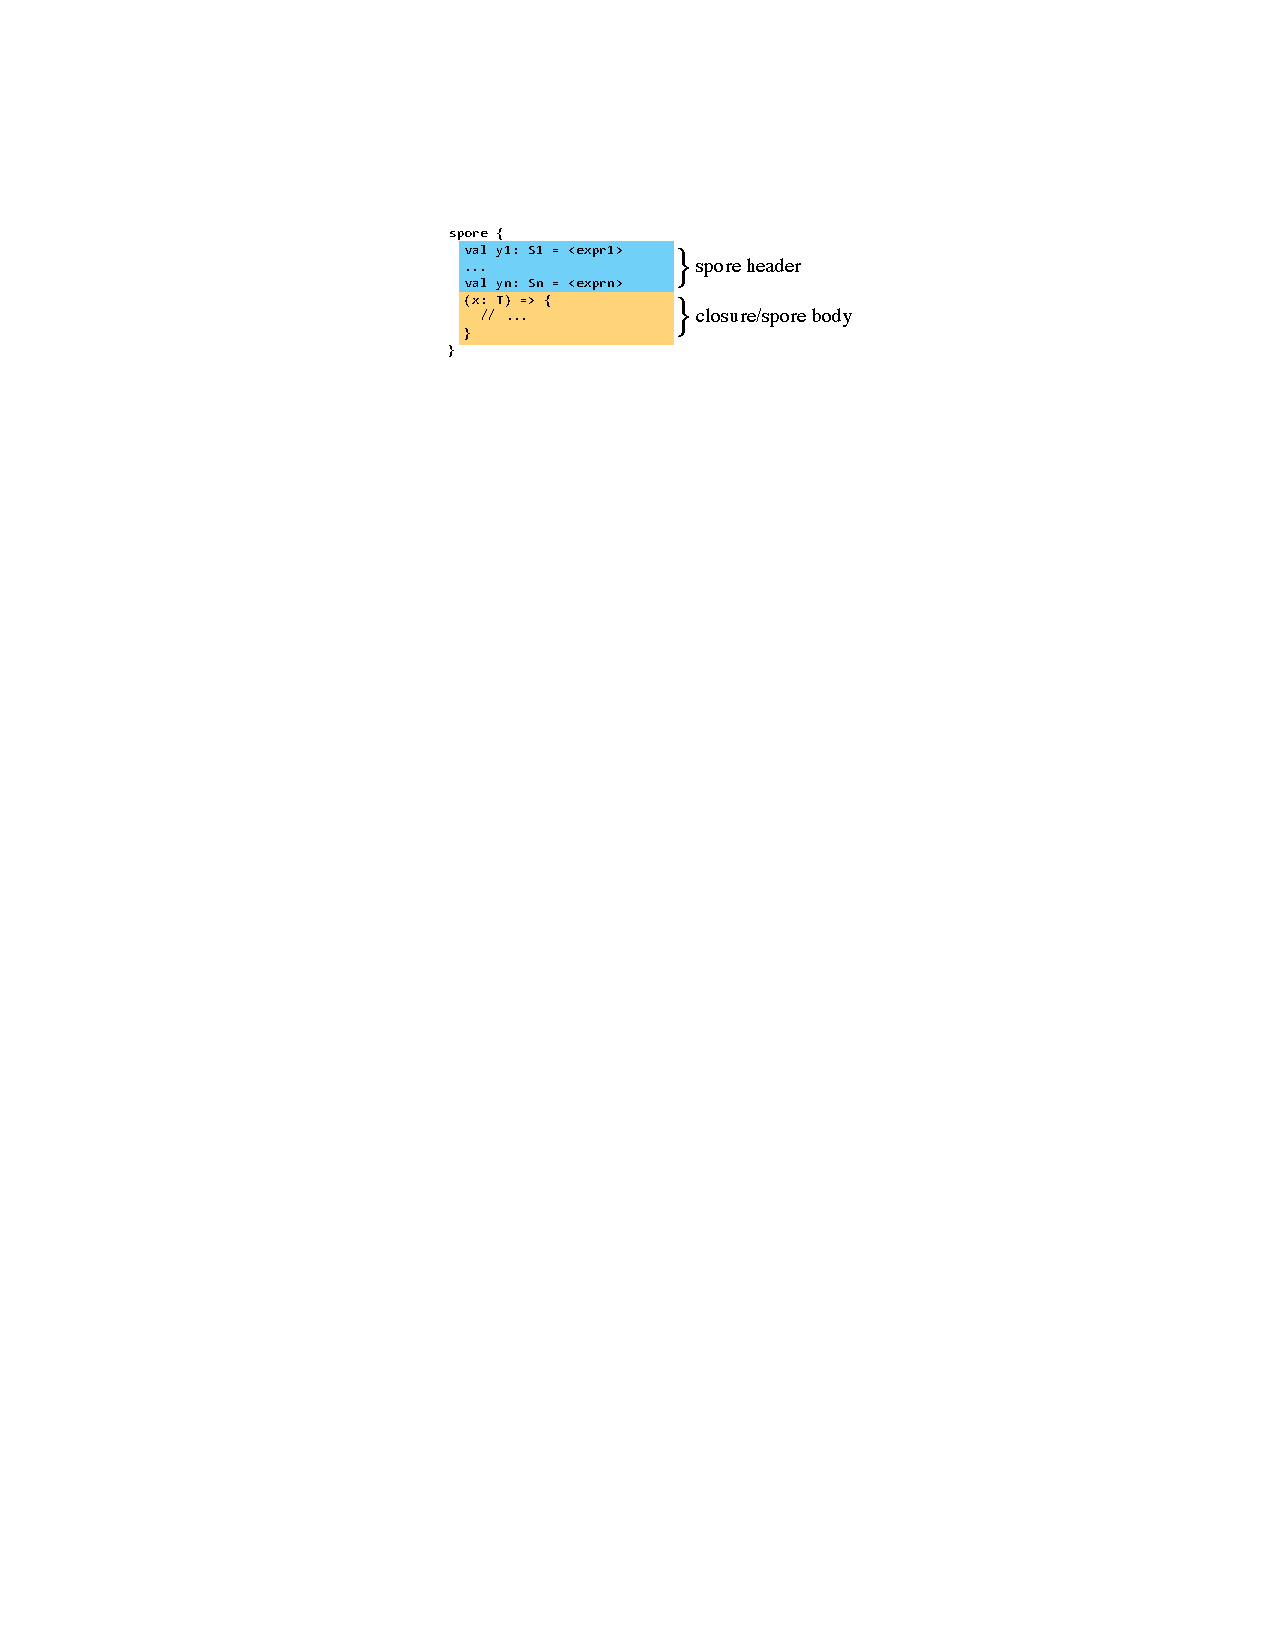
\includegraphics[width=0.75\columnwidth]{spore-shape.pdf}
\end{figure}
\vspace{-1mm}

The characteristic property of a spore is that the spore body is only allowed
to access its parameter, the values in the spore header, as well as top-level
singleton objects (Scala's form of modules). The spore closure is not allowed
to capture variables other than those declared in the spore header (\ie a
spore may not capture variables in the environment). By enforcing this shape,
the environment of a spore is always declared explicitly in the spore header,
which avoids accidentally capturing problematic references. Moreover,
importantly for object-oriented languages like Scala, it's no longer possible
to accidentally capture the \verb|this| reference.

Spores also come with additional type-checking. Type information corresponding
to captured variables are included in the type of a spore. This enables
authors of distributed frameworks to customize type-checking of spores to, for
example, {\em exclude} a certain type from being captured by user-provided
spores. Authors of distributed frameworks may kick on this type-checking by
simply including information about excluded types (or other type-based
properties) in the signature of a method. A concrete example would be to
ensure that the \verb|map| method on \verb|RDD|s in Spark to accept only
spores which do not capture \verb|SparkContext| (a non-serializable internal
framework class).

For a deeper understanding, see either Appendix~\ref{appendix:spores} which
covers the semantics of spores or the corresponding publication~\cite{Spores}.

\begin{figure}[t!]
\centering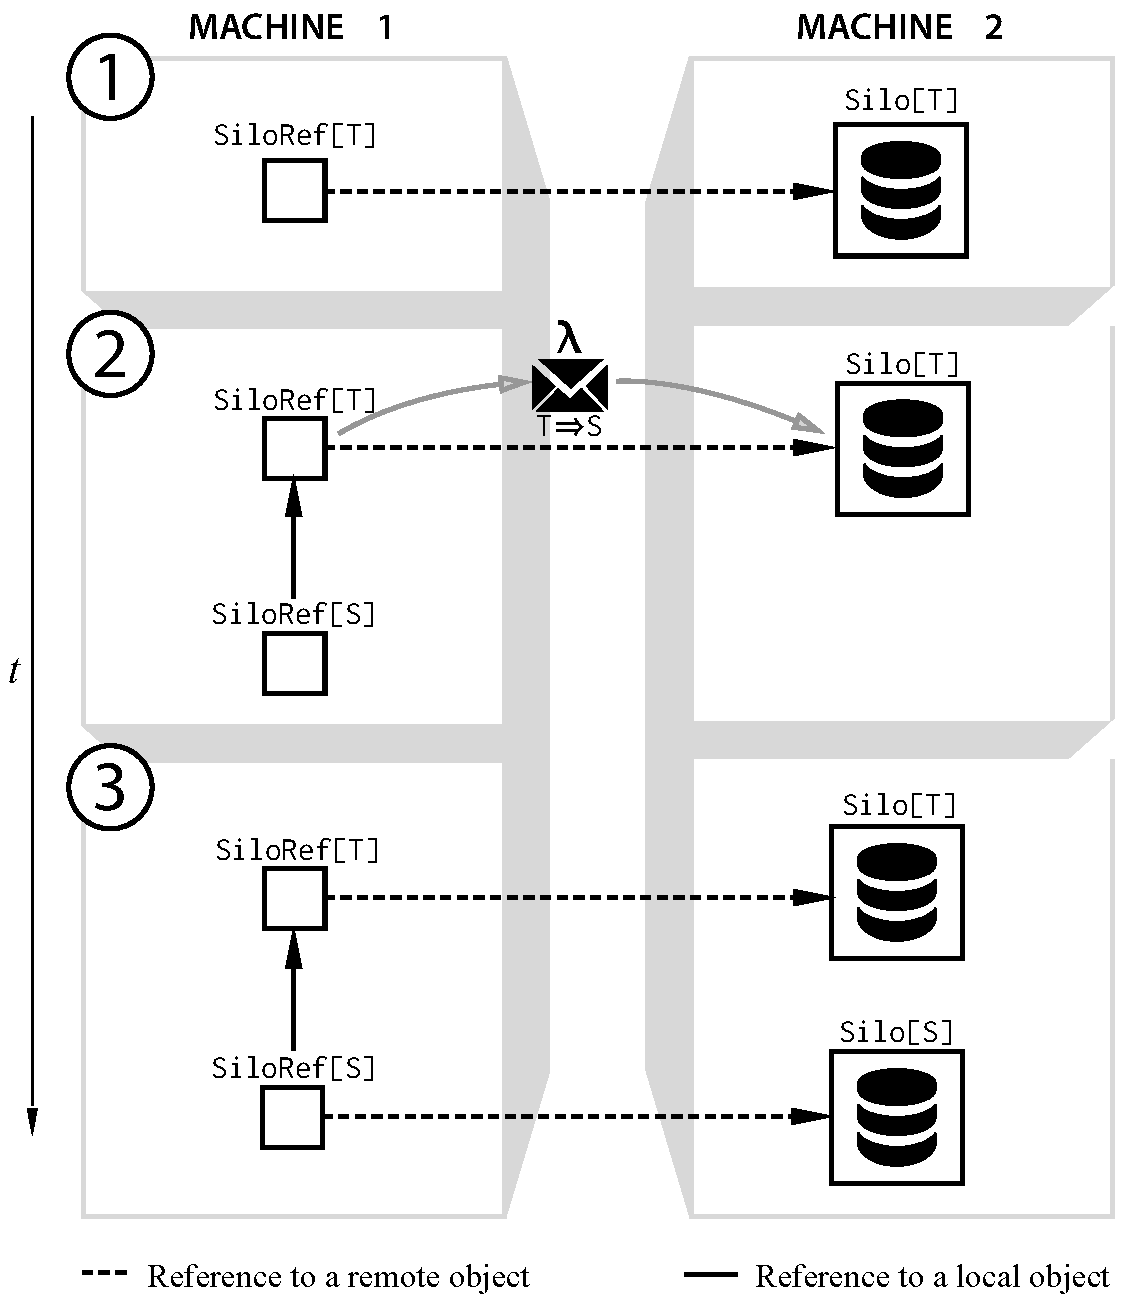
\includegraphics[width=0.8\columnwidth]{basic-diagram.pdf}
\caption{Basic model.}\label{fig:basic-diagram}
\end{figure}

\subsection{Basic Usage}

The only way to interact with distributed data stored in silos is through the
use of SiloRefs. A SiloRef can be thought of as an immutable handle to the
remote data contained within a corresponding silo. Users interact with this
distributed data by applying functions to SiloRefs, which are transmitted over
the wire and later applied to the data within the corresponding silo. As is
the case for persistent data structures, when a function is applied to a piece
of distributed data via a SiloRef, a new SiloRef representing the transformed
data is returned.

The simplest illustration of the model is shown in Figure~\ref{fig:basic-diagram}
(time flows vertically from top to bottom). Here, we start with a
\verb|SiloRef[T]| which points to a piece of remote data contained within a
\verb|Silo[T]|. When the function shown as $\lambda$ of type $T \Rightarrow S$
is applied to \verb|SiloRef[T]| and ``forced'' (sent over the wire), a new
SiloRef of type \verb|SiloRef[S]| is immediately returned. Note that
\verb|SiloRef[S]| contains a reference to its parent SiloRef,
\verb|SiloRef[T]| (This is how {\em lineages} are constructed). Meanwhile, the
function is asynchronously sent over the wire and is applied to
\verb|Silo[T]|, eventually producing a new \verb|Silo[S]| containing the data
transformed by function $\lambda$. This new \verb|SiloRef[S]| can be
used even before its corresponding silo is materialized (\ie before the data
in \verb|Silo[S]| is computed) – the F-P framework queues up operations
applied to \verb|SiloRef[S]| and applies them when \verb|Silo[S]| is fully
materialized.

Several vastly different sorts of complicated DAGs can be asynchronously built
up this way. Though first, to see how this is possible, we need to develop a
clearer idea primitive operations available on SiloRefs and their semantics.
We describe these in the following section.


\subsection{Primitives}
\label{sec:primitives}

There are four basic primitive operations on SiloRefs that together can be
used to build the higher-order operations common to popular data-centric
distributed systems (how to build some of these higher-order operations is
described in Section~\ref{sec:higher-order-operations}). These primitives
include:

\begin{itemize}[noitemsep,nolistsep]
\item \verb|map|
\item \verb|flatMap|
\item \verb|send|
\item \verb|cache|
\end{itemize}

\paragraph{map}
The \verb|map| method takes a spore that is to be applied to the data in the
silo of the receiver SiloRef. Rather than immediately sending the spore across
the network, and waiting for the operation to finish, the \verb|map| method is
\emph{lazy}. Without involving any network communication, it immediately
returns a SiloRef referring to a new, lazily-created silo. This new SiloRef
only contains lineage information, namely, a reference to the original
SiloRef, a reference to the argument spore, and the information that it is the
result of a \verb|map| invocation. (The \verb|send| method is used to force
the materialization of the result silo, see below.) For example, given a silo
with a list of \verb|Person| records, the following application of \verb|map|
defines a silo containing only the records of adults:

\begin{lstlisting}
val persons: SiloRef[List[Person]] = ...
val adults = persons.map(spore { ps => ps.filter(p => p.age >= 18) })
\end{lstlisting}

\paragraph{flatMap}
Like \verb|map|, the \verb|flatMap| method takes a spore that is to be applied
to the data in the silo of the receiver SiloRef. However, the crucial
difference is in the type of the spore argument whose result type is a SiloRef
in this case. Semantically, the new silo created by \verb|flatMap| is defined
to contain the data of the silo that the user-defined spore returns. The
\verb|flatMap| combinator adds expressiveness to our model that is essential
to express more interesting computation DAGs. For example, consider the
problem of combining the information contained in two different silos
(potentially located on different hosts). Suppose the information of a silo
containing \verb|Vehicle| records should be enriched with other details only
found in the \verb|adults| silo. In the following, \verb|flatMap| is used to
create a silo of \verb|(Person, Vehicle)| pairs where the names of person and
vehicle owner match:

\begin{lstlisting}
val vehicles: SiloRef[List[Vehicle]] = ...
// adults that own a vehicle
val owners = adults.flatMap(spore {
  val localVehicles = vehicles // spore header
  ps =>
    localVehicles.map(spore {
      val localps = ps // spore header
      vs =>
      localps.flatMap(p =>
        // list of (p, v) for a single person p
        vs.flatMap { v =>
          if (v.owner.name == p.name) List((p, v))
          else List()
        }
      )
    })
})
\end{lstlisting}

Note that the spore passed to \verb|flatMap| declares the capturing of the
\verb|vehicles| SiloRef in its so-called ``spore header''. The spore header
spans all variable definitions between the spore marker and the parameter list
of the spore's closure. The spore header defines the variables that the
spore's closure is allowed to access. Essentially, spores limit the free
variables of their closure's body to the closure's parameters and the
variables declared in the spore's header. Within the spore's closure, it is
necessary to read the data of the \verb|vehicles| silo in addition to the
\verb|persons| list. This requires calling \verb|map| on \verb|localVehicles|.
However, \verb|map| returns a SiloRef; thus, invoking \verb|map| on
\verb|adults| instead of \verb|flatMap| would be impossible, since there would
be no way to get the data out of the silo returned by
\verb|localVehicles.map(..)|. With the use of \verb|flatMap|, however, the
call to \verb|localVehicles.map(..)| creates the final result silo, whose data
is then also contained in the silo returned by \verb|flatMap|.

Clearly, \verb|map| can be expressed in terms of \verb|flatMap|:

\begin{lstlisting}
def map[S](s: Spore[T, S]): SiloRef[S] = {
  this.flatMap(spore {
    val localSpore = s
    x =>
      val res = localSpore(x)
      SiloRef.fromFun(currentHost)(spore {
        val localRes = res
        () => localRes
      })
}
\end{lstlisting}

This should come as no surprise, given that \verb|flatMap| is the monadic bind
operation on SiloRefs, and \verb|SiloRef.fromFun|\todo{fromFun is now introduced later. fix this} is the monadic return
operation. The reason why \verb|map| is provided as one of the main operations
of SiloRefs is that direct uses of \verb|map| enable an important optimization
based on operation fusion. This optimization is explained following the
discussion of the third main operation of SiloRefs, \verb|send|.

\paragraph{send}
The final operation of SiloRefs is \verb|send|. It forces the lazy computation
defined by the given SiloRef. Forcing is explicit in our model, because it
requires sending the lineage to the remote node on which the result silo
should be created. Given that network communication has a latency several
orders of magnitude greater than accessing a word in main memory, say, we felt
an explicit send operation a judicious choice. To enable materialization of
remote silos to proceed concurrently, the \verb|send| operation immediately
returns a future. This future is then asynchronously completed with the data
of the given silo. Since calling \verb|send| will materialize a silo and send
its data to the current node, \verb|send| should only be called on silos with
reasonably small data. For example, Figure ?? shows the effect of invoking
\verb|send| on the \verb|labels| SiloRef from above.

The \verb|send| operation can also be used to simply cache a silo in main
memory, for example, because the silo is known to be accessed subsequently:

\begin{lstlisting}
def cache(): Future[Boolean] = this.flatMap(spore {
  val localDoneSiloRef = DoneSiloRef
  res => localDoneSiloRef.send()
}
\end{lstlisting}

\paragraph{cache}
The \verb|cache| method can be provided for convenience. It invokes
\verb|send| not directly on the given SiloRef (which would transfer all data
of the silo to the current node); instead, it first uses \verb|flatMap| to
create a new silo that will be completed with the trivial value (e.g., a
Boolean constant) of the \verb|DoneSiloRef| singleton object. Essentially,
invoking \verb|send| on this trivial SiloRef causes the resulting future to be
completed as soon as \verb|this| SiloRef has been materialized in main memory.



\subsection{Creating Silos}
\label{sec:creating-silos}

Besides a type definition for SiloRef, our framework also provides a companion
singleton object (Scala's form of modules). The singleton object provides
factory methods for obtaining SiloRefs referring to silos populated with some
initial data:\footnote{The given code snippets are minimally simplified for
clarity. No essential details are omitted.}

\begin{lstlisting}
object SiloRef {
  def fromTextFile(host: Host)(file: File): SiloRef[List[String]] = ...
  def fromFun[T](host: Host)(s: Spore[Unit, T]): SiloRef[T] = ...
}
\end{lstlisting}

Each of the factory methods has a \verb|host| parameter that specifies the
target host (address/port) on which to create the silo. Note that the
\verb|fromFun| method takes a spore closure as an argument to make sure it can
be serialized and sent to \verb|host|. In each case, the returned SiloRef
contains its \verb|host| as well as an identifier that uniquely identifies its
silo on the \verb|host|. To obtain this host-unique identifier, each factory
method has to communicate with the target \verb|host|.

The type \verb|SiloRef[T]| has the following main operations:

\begin{lstlisting}
trait SiloRef[T] {
  def map[S](s: Spore[T, S]): SiloRef[S]
  def flatMap[S](s: Spore[T, SiloRef[S]]): SiloRef[S]
  def send(): Future[T]
}
\end{lstlisting}


Nothing beats a video when something evolves in space in time, so we've also produced a short video to illustrate the model\footnote{\url{https://vimeo.com/120415626}}


\subsection{Fault Handling}
\label{sec:fault-handling}

Besides the primitives discussed so far, the programming model includes
overloaded variants that enable the definition of flexible fault handling
semantics. The main idea is to specify fault handlers for \emph{subgraphs of
computation DAGs}. Our guiding principle is to make the definition of the
failure-free path through a computation DAG as simple as possible, while still
enabling the handling of faults at the fine-granular level of individual
SiloRefs.

\paragraph{Defining fault handlers} Fault handlers may be specified whenever
the lineage of a SiloRef is extended. For this purpose, the introduced
\verb|map| and \verb|flatMap| primitives are overloaded. For example,
consider our previous example, but extended with a fault handler:

\begin{lstlisting}
val persons: SiloRef[List[Person]] = ...
val vehicles: SiloRef[List[Vehicle]] = ...
// copy of `vehicles` on different host `h`
val vehicles2 = SiloRef.fromFun(h)(spore {
  val localVehicles = vehicles
  () => localVehicles
})

val adults =
  persons.map(spore { ps => ps.filter(p => p.age >= 18) })

// adults that own a vehicle
def computeOwners(v: SiloRef[List[Vehicle]]) =
  spore {
    val localVehicles = v
    (ps: List[Person]) => localVehicles.map(...)
  }

val owners: SiloRef[List[(Person, Vehicle)]] =
  adults.flatMap(computeOwners(vehicles),
                 computeOwners(vehicles2))
\end{lstlisting}

Importantly, in the \verb|flatMap| call on the last line, in addition to
\verb|computeOwners(vehicles)|, the regular spore argument of \verb|flatMap|,
\verb|computeOwners(vehicles2)| is passed as an additional argument. The
second argument registers a \emph{failure handler} for the subgraph of the
computation DAG starting at \verb|adults|. This means that if during the
execution of \verb|computeOwners(vehicles)| it is detected that the
\verb|vehicles| SiloRef has failed, it is checked whether the SiloRef that the
higher-order combinator was invoked on (in this case, \verb|adults|) has a
failure handler registered. In that case, the failure handler is used as an
alternative spore to compute the result of \verb|adults.flatMap(..)|. In this
example, we specified \verb|computeOwners(vehicles2)| as the failure handler;
thus, in case \verb|vehicles| has failed, the computation is retried using
\verb|vehicles2| instead.





\section{Higher-Order Operations}
\label{sec:higher-order-operations}

Operations on distributed collections\todo{somehow mention Spark here so it's
clear what a dist coll is.}~such as \verb|union|, \verb|groupByKey|, or
\verb|join|, involve multiple data sets, possibly located on different nodes.
In the following we explain how such operations can be expressed using the
introduced primitives.\todo{need a more compelling into for PL people}

\paragraph{union}
The union of two unordered collections stored in two different silos can be
expressed directly using the above \verb|flatMap| primitive.

\paragraph{join}
Suppose we are given two silos with the following types:

\begin{lstlisting}
val silo1: SiloRef[List[A]]
val silo2: SiloRef[List[B]]
\end{lstlisting}

\noindent as well as two hash functions computing hashes for elements of
type \verb|A| and \verb|B|, respectively:

\begin{lstlisting}
val hashA: A => K = ...
val hashB: B => K = ...
\end{lstlisting}

The goal is to compute the hash-join of \verb|silo1| and \verb|silo2|:

\begin{lstlisting}
val hashJoin: SiloRef[List[(K, (A, B))]] = ???
\end{lstlisting}

To be able to use \verb|flatMap|, the types of the two silos first have to be
made equal, through initial \verb|map| invocations:


\begin{lstlisting}
val silo12: SiloRef[List[(K, Option[A], Option[B])] =
      silo1.map { x => (hashA(x), Some(x), None) }
val silo22: SiloRef[List[(K, Option[A], Option[B])] =
      silo2.map { x => (hashB(x), None, Some(x)) }
\end{lstlisting}

Then, we can use \verb|flatMap| to create a new silo (at some destination
place), which contains the elements of both \verb|silo12| and \verb|silo22|:

\begin{lstlisting}
val combined = SiloRef.flatMap(destPlace, silo12, silo22,
                              (elem, emitter) => emitter.emit(elem),
                              listBuilderFactory[...])
\end{lstlisting}

The combined silo contains triples of type \verb|(K, Option[A], Option[B])|.
Using an additional \verb|map|, the collection can be sorted by key, and adjacent
triples be combined, yielding a \texttt{SiloRef[List[(K, (A, B)} as required.


\paragraph{Partitioning and groupByKey}

A \verb|groupByKey| operation on a group of silos containing collections needs
to create multiple result silos, on each node, with ranges of keys supposed to
be shipped to destination nodes. These destination nodes are determined using
a partitioning function. Our goal, concretely:

\begin{lstlisting}
val groupedSilos = groupByKey(silos)
\end{lstlisting}

Furthermore, we assume that \verb|silos.size| $= N$ where $N$ is the number of
nodes, with nodes $N_1$, $N_2$, etc. We assume each silo contains an unordered
collection of key-value pairs (a multi-map). Then, \verb|groupByKey| can be
implemented as follows:

\begin{itemize}
\item For each node $N_i$, the master node creates $N$ SiloRefs.

\item Each node $N_i$ applies a {\em partitioning function}
(example: \texttt{hash(key) mod N}) to the key-value pairs in its silo,
yielding $N$ (local) silos.

\item Using \verb|flatMap|, each pair of silos containing keys of the
same range can be combined and materialized on the right destination node.
\end{itemize}

\section{Formalization}
\label{sec:formalization}

\section{Implementation}
\label{sec:implementation}

\section{Evaluation}
\label{sec:evaluation}

\section{Related Work}
\label{sec:related-work}

\section{Conclusion and Future Work}
\label{sec:conclusion-future-work}

Actors~\cite{Actors, ScalaActors}. Typed Actors~\cite{TypedActors}. MapReduce~\cite{MapReduce}. Spark~\cite{Spark}. Dryad~\cite{Dryad}. Session Types~\cite{SessionTypes}. Cloud Haskell~\cite{CloudHaskell}. Alice ML~\cite{AliceML}. Acute ML~\cite{AcuteML}. Type-safe distributed OCaml~\cite{DistOCaml}. AmbientTalk~\cite{AmbientTalk}. E Language~\cite{ELang}. Clojure's Agents~\cite{Clojure}.


\section{Old}

\subsection{Old Intro}

% From the ivory tower, it may not be evident,
% It might not seem this way from the ivory tower,
% but

While it might not seem that way at a glance, mainstream software development
has become largely distributed. Two {\em styles} of distribution
dominate the current landscape; (1) systems composed of microservices,
 % or designed to be software as a service (SaaS),
and (2) systems for ``big data'' processing. Names like Netflix, SoundCloud,
and Twitter have established their competitive offerings by way of one or
both of these types of systems.

Microservices are small, independent (separately-compiled) services running on
different machines which communicate with each other to together make up a
single and complex application. ``Big data''-style applications on the other
hand are typically single applications whose data cannot fit into the memory
of one machine alone. Such applications are typically singly-compiled, with
their binaries distributed across a cluster of machines.

Yet, software developers still fumble with low-level RPC frameworks.
% and sluggish serialization frameworks.
Mainstream programming languages have traditionally offered little support in
this space.

We design module systems, etc, for maximum reuse and productivity, we go as
far as we can to demonstrate their power. But we often . Some of these
concerns have been affectionately referred to as the ``awkward
squad''~\cite{AwkwardSquad} by PL research, and they are concerns that are central to
contemporary software development.

Functional programming brings value to distributed systems builders. The
success of popular Spark can be attributed to functional ideas.

However, beyond Spark's interface, .

We refer to the model as {\em function-passing}, and .


We design a programming model in such a way that we can ``maximize'' static
types, and with it enable type-specialized picklers (statically generated),
typed closures, and type-specialized data structures.

The motto is ``making type inference work for you when optimizing distributed
systems'', or ``how type inference and existential types benefit distributed
systems''.

In existing systems, types are only in the user-facing API and help the user.
However, all too often, the internals of a distributed system are largely
untyped, in particular when operating on data types that are also shipped
remotely. In our approach we now go ahead and make types work so that they
benefit both users (helping catch common errors) \emph{and} distributed
systems builders. Our approach leverages types to provide (1) type-specialized
picklers, and (2) type-specialized collections/builders.

The approach is novel, because noone talks about making sure the unpicklers
and builders themselves are serializable, but that's actually fundamental to
the whole design.

\begin{itemize}

\item We have to make the point that serialization is like a primitive in
systems design, not some extra thing you figure out how to do later, like in
typical PLs. so maybe one central point that we should try to make is that
for distributed systems, serializability is like a key primitive, along with
latency and other things.

\item we want to prove that typed distributed systems are a good idea. right
now a lot of systems for dist computing are fundamentally untyped or
dynamically checked. those that are typed lose type information between
machines.

\item so we're trying to argue that types are good for system builders.

\end{itemize}

The fact that actually these benefits from types \emph{carry over to other
models as well} (not just spark-like models).


Generalization of MapReduce model. Low-level. Inversion of the actor model.
Can represent different many models for distributed computing, e.g. Spark,
Percolator (we probably can't validate this claim.)

Illustrations to have:
\begin{enumerate}
\item nice figure
\item organic evolving model on youtube
\end{enumerate}

\subsection{Evaluation}

we could make the performance eval strong by saying, ok, we implemented real
apps, so we have the real communication that needs to happen (and happens).
and we now make this communication typed, plus we measure exactly the
percentage of time that's spent in serialization for example. and then we
could even interpolate the results, so we could say, ok, if some other dist
system has a lower percentage spent in serialization, then the speed up would
be like this.

and then we could even measure that for real spark, and then interpolate and
say, ok, in the ideal case, meaning using all of our design principles, we
could speed up things like this, if one would re-architect spark to preserve
types (it's a huge task, so out of scope).

well, it would definitely be something that we can measure objectively. the
only thing we have to guard against would be to say, adding picklers and
builders does not otherwise \emph{degrade} performance, like, we'd have to
prove that there's no cost, but \emph{just} the performance benefits. adding
the classname of the unpickler adds a few bytes to each pickle, for example.

we could even show that with babyspark, like have a version that uses java
serialization, then a version that uses pickling without selfdescribing, then
with runtime unpickling, and with all static. because we have those numbers
for babyspark then the interpolation will be much more precise.



\section{Future Work}

Adapt this model for streaming computation. This would take coming up with a
solution to null out references in the {\em lineage}. This would make it possible to instantiate and populate new silos to handle incoming data.

\appendix
\section{Spores}
\label{appendix:spores}

% This is the text of the appendix, if you need one.

% \acks

% Acknowledgments, if needed.

% We recommend abbrvnat bibliography style.

\bibliographystyle{abbrvnat}

% The bibliography should be embedded for final submission.
\bibliography{bib}

% \begin{thebibliography}{}
% \softraggedright

% \bibitem[Smith et~al.(2009)Smith, Jones]{smith02}
% P. Q. Smith, and X. Y. Jones. ...reference text...

% \end{thebibliography}


\end{document}

%                       Revision History
%                       -------- -------
%  Date         Person  Ver.    Change
%  ----         ------  ----    ------

%  2013.06.29   TU      0.1--4  comments on permission/copyright notices

